\documentclass[12pt]{article}
\usepackage{listings}

\usepackage[utf8]{inputenc}
%\usepackage[T1]{fontenc}
\lstset{frame=tb,
  aboveskip=3mm,
  belowskip=3mm,
  showstringspaces=false,
  columns=flexible,
  basicstyle={\small\ttfamily},
  breaklines=true,
  breakatwhitespace=true,
  tabsize=2
}
\usepackage{geometry}
\geometry{a4paper}
\usepackage{graphicx}
\usepackage{float}
\usepackage[italian]{babel}

\linespread{1.2}
\setlength{\parindent}{0pt}

\begin{document}

%----------------------------------------------------------------------------------------
%	TITOLO
%----------------------------------------------------------------------------------------

\begin{titlepage}

\newcommand{\HRule}{\rule{\linewidth}{0.5mm}}
\center

\textsc{\Large Relazione di progetto di Laboratorio di Sistemi Software}\\[0.5cm]

\HRule \\[0.4cm]
{ \huge \bfseries Trasporti 116117 - Digital Twin}\\[0.4cm]
\HRule \\[1.5cm]

\vfill

\begin{flushleft}
\emph{Gibertoni Giada, Galassi Meshua}\\[3cm]

\end{flushleft}



\end{titlepage}

%----------------------------------------------------------------------------------------
%	INDICE
%----------------------------------------------------------------------------------------

\tableofcontents

\newpage

\section{Obiettivo del progetto}
Il progetto consiste nello studio e nell'implementazione di una serie opportuna di digital twins in un contesto di gestione in ambito healthcare.
In particolare, si tratta di un progetto che mira ad un miglioramento della gestione dei trasporti ospedalieri secondari, ovvero, uno dei servizi forniti dal numero unico europeo 116117 adibito alle cure mediche non urgenti ed altri servizi territoriali a bassa priorità.
Ci si focalizzerà quindi, ad esempio, sui trasferimenti casa - ospedale e viceversa, oppure, sui trasporti tra strutture ospedaliere.

Si è scelto di applicare il paradigma dei digital twins al fine di riportare una rappresentazione digitale del mondo reale in modo da facilitare l'analisi dello stato attuale del servizio fornito e una migliore comprensione di quali potrebbero essere i miglioramenti da apportare. 

\section{Domain Driven Design}

\subsection{Fase di Knowledge Crunching}
Il numero unico europeo 116117 è un servizio telefonico che permette di accedere a cure mediche non urgenti ed altri servizi sanitari territoriali a bassa priorità.
Il servizio si rivolge a tutti i cittadini, italiani o stranieri, in maniera totalmente gratuita e fruibile da qualsiasi apparecchio, senza richiedere una registrazione preventiva.
\`E un numero a chiamata rapida, non necessita di prefisso ed è disponibile 24 ore al giorno per 7 giorni alla settimana per fornire assistenza o informazioni.
Attraverso il numero 116117 si gestiscono diversi settori:
\begin{enumerate}
    \item Medico Continuità Assistenziale: è un servizio che permette di filtrare le chiamate ai medici per le visite domiciliari, alle USCA, alla guardia medica turistica ed alla centrale operativa 118.
    \item Centrale trasporti secondari: permette agli operatori di coordinare i trasporti secondari dell'AUSL Romagna, in modo da consentire una più efficiente gestione dei mezzi di trasporto nei vari ambiti. 
    \item Infermiere di territorio: ha l'obiettivo di fornire informazioni agli utenti e svolgere funzioni utili al monitoraggio ed all'assistenza in telemedicina.
    \item Telemedicina: monitoraggio di pazienti a domicilio attraverso sistemi di trasmissione dati che consentono una valutazione dello stato di salute del paziente in modo da fornire, se necessario, risposte sanitarie urgenti.
\end{enumerate}

In questo progetto, ci focalizzeremo sulla gestione della centrale dei trasporti secondari con lo scopo di rendere più efficiente il servizio fornito attualmente. In particolare, si vorrà rendere possibile un tracciamento dei mezzi di trasporto per migliorare la loro efficienza e sfruttamento ed evitare situazioni che portano ad uno spreco delle risorse disponibili.
Inoltre, si vuole rendere possibile il tracciamento e il monitoraggio di tutti gli eventi rilevanti relativi ai trasporti secondari, così da produrre report e studiare l'andamento del servizio tramite indicatori statistici e KPI.
Il sistema, potrebbe essere utile per costruire simulazioni di situazioni reali per aiutare la pianificazione e la gestione delle risorse.

\textbf{Normativa trasporti sanitari}
In materia di trasporti secondari esistono diverse normative di seguito riportate:

\begin{itemize}
    \item \textbf{DM 70/2015} definisce gli standard qualitativi, strutturali e tecnologici da seguire per garantire una assistenza ospedaliera.
    Deve essere previsto lo sviluppo del servizio di emergenza territoriale tecnologicamente avanzato in modo tale da garantire una reale continuità dell'assistenza, anche attraverso la gestione tempestiva dei trasferimenti secondari urgenti in carico al 118 e la trasmissione di immagini e dati.
    Il DM sottolinea il fatto che sia nel caso in cui la gestione e il fabbisogno di mezzi dei trasporti secondari siano affidati a presidi ospedalieri, sia nel caso in cui siano affidati al 118 devono essere mantenuti separati dalla gestione del servizio di soccorso sanitario urgente.
    \item \textbf{DPCM 12 dicembre 2017} stabilisce che il sistema sanitario nazionale garantisca interventi sanitari tempestivi assicurando il trasporto in condizioni di sicurezza al presidio ospedaliero più appropriato.
    \item \textbf{Legge 17 luglio 2020, n. 77} stabilisce che, a causa dell'emergenza Covid-19, le regioni e le province autonome possano aumentare il numero di mezzi ed il relativo personale necessario per sostenere i trasporti secondari per pazienti Covid-19, per le dimissioni protette e per i trasporti interospedalieri di pazienti non affetti da Covid-19.
    \item \textbf{Regolamenti AUSL della Romagna} sottolinea che a causa dell'assenza di indicazioni regionali i trasporti secondari vengono gestiti in maniera diversa tra le varie aziende e anche all'interno di ognuna tra i diversi ambiti. Questo ha un effetto negativo poiché spesso in alcuni ambiti sono garantiti trasporti di un certo tipo e in altri no, questo varia il fabbisogno dei mezzi in maniera significativa.
\end{itemize}

\textbf{Situazione attuale AUSL della Romagna}

All'interno di AUSL della Romagna vi sono tre centrali operative per i trasporti secondari, di cui soltanto una è operativa h24. Queste centrali non sono collegate tra loro e con la centrale del 118, se non per telefono; questo causa una forte disomogeneità che comporta inefficienze rilevanti come ad esempio gestione dei mezzi per ambito e senza fare considerazioni di tipo geografico.
Inoltre, a causa della non continuità del servizio, può capitare che le richieste effettuate dopo l'orario di chiusura del sistema di prenotazione, vengano passate alla centrale operativa 118 utilizzando ambulanze destinate all'emergenza territoriale.

Elementi di criticità:
\begin{itemize}
    \item Assenza di un software unico tra le varie centrali con conseguenti difficoltà organizzative.
    \item Assenza di una rete radio unica con difficoltà di comunicazione tra le centrali ed i mezzi tra ambiti diversi.
    \item Aumento dei costi progressivo senza evidenti benefici per il sistema.
    \item Assenza di tracciabilità degli spostamenti con conseguente difficoltà nel tracciare i tempi degli stessi.
\end{itemize}

\textbf{Proposta di riorganizzazione}

 \begin{figure}[!ht]
    \centering
      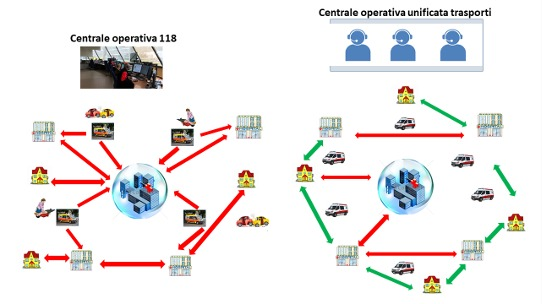
\includegraphics[width=13cm]{fig/modelloIdeale.jpeg}
      \caption{Modello ideale centrale operativa 118 e centrale operativa unificata trasporti}
      \label{modello_ideale}
    \end{figure}
    
Seguendo anche quanto previsto dal DM 70/2015, si individuano due sistemi distinti:
\begin{itemize}
    \item Sistema di emergenza sanitaria territoriale gestita dalla centrale operativa 118 che si occupa solamente dei servizi di emergenza (il suo lavoro si conclude, ove necessario, con il primo trasporto in ospedale).
    \item Sistema trasporti sanitari gestito dalla centrale unificata trasporti che si occupa solamente dei trasporti non in emergenza. Riguarda tutti i trasporti interospedalieri e gli altri trasporti da e verso il domicilio o altre strutture.
\end{itemize}
    
Nella realtà può accadere che il primo ospedale di destinazione non sia quello idoneo e che si rilevi la necessità di trasferimento del paziente in un altro ospedale. Poiché si tratta di un trasferimento a carico dei trasporti secondari ma non programmato, il trasporto potrebbe non essere disponibile e potrebbe essere necessario rivolgersi al 118. La sinergia tra i due sistemi è un elemento di forza per rispondere meglio alle esigenze: è necessario un'organizzazione che tenga conto di entrambi i sistemi, per evitare inefficienze, sovrapposizioni e ritardi.

Il modello proposto prevede inizialmente il mantenimento delle tre centrali separate ma, unificate a livello organizzativo. In un futuro si vorrebbe creare un'unica centrale operativa per i trasporti secondari come riportato in figura \ref{modello_ideale}.

\subsubsection{Incontro con l'esperto del dominio - 19.03.2021}
All'inizio della call il Dottor Menarini spiega com'è nata la gestione delle emergenze/urgenze sanitarie, i trasporti secondari e la guardia medica. Inizialmente nacquero come un unico sistema, ovvero i trasporti secondari erano gestiti dallo stesso 118. Successivamente furono gestiti in maniera distaccata in quanto ritenuti servizi meno importanti ed ora hanno vita propria e sono divise per ambito con varie inefficienze. 

Con la comparsa del Covid-19 ci si rende conto che manca un interfaccia tra territorio ed ospedale; il 118 si è dovuto prendere carico anche di situazioni che di fatto non erano di emergenza, ad esempio per informazioni o paura dei cittadini.

Oltre al 118, andrebbero sviluppati molti altri settori come trasporti, telemedicina e teleassistenza che ancora sono mal gestiti o assenti.
Il vantaggio derivante dallo sviluppo di questi settori è quello di avere un collegamento tra cittadino e assistenza sanitaria. Attraverso questa interfaccia si potrebbero dare risposte migliori e indirizzare al meglio il cittadino e, in alcuni casi, intercettare prima i bisogni di quest'ultimo. 

Considerando la situazione sanitaria attuale uno dei settori più in sofferenza è proprio quello che dovrebbe essere gestito dal 116117 poiché non è stato progettato in precedenza.

Il 112 dovrebbe essere utilizzato per le emergenze e il 116117 per le non emergenze. 
Nel momento in cui le chiamate non sono indirizzate al giusto centralino, vengono reindirizzate a quello di competenza, poiché le centrali saranno distaccate fisicamente ma interdipendenti tra loro. Questo è un elemento da considerare in fase progettuale. 

Già dal 2013 nel decreto rilancio era presente un comma che faceva riferimento alle centrali regionali con il 116117, ma soltanto dopo 8 anni e l'emergenza Covid-19 se ne è capita davvero l'importanza.
\hfill \break

Per quanto riguarda la dotazione dei mezzi di trasporto, nel modello idealizzato del passato erano previsti due sottosistemi, ovvero il trasporto con ambulanze e le emergenze con ambulanze. Questi sottosistemi hanno sempre vissuto in maniera separata ma si è resa evidente l'esigenza che l'uno si debba interfacciare con l'altro per questo servirebbero dei mezzi equipotenti (soprattutto per quanto riguarda la trasmissione dati), tenuti comunque separati a livello tecnico ma intercambiabili e interfacciabili tra loro.
Un esempio di situazione in cui sorge questa necessità, è il caso in cui si esauriscano i mezzi per le emergenze e debbano essere utilizzati al loro posto i mezzi adibiti ai trasporti secondari che però, al momento, non sono equipaggiati a dovere.

Attualmente i mezzi del 118 sono equipaggiati con tablet in connessione con la centrale operativa. Per quello che riguarda i trasporti secondari, non c'è ancora una tracciabilità dei mezzi, ci sono soltanto sistemi di radiocomunicazione e le chiamate viaggiano su telefono. Si può presupporre comunque, la possibilità di avere un tablet associato al mezzo secondario e che i professionisti che usano questi mezzi siano dotati di un proprio tablet/smartphone associato al ruolo e non al mezzo.
\hfill \break

Durante la call è stato richiesto all'esperto del dominio di fornire alcune user story per comprendere meglio il dominio. Si sono identificati tre assi principali: chiamata di emergenza standard, trasporto standard e chiamata che non rientra in nessuno dei due casi precedenti.
Alcuni scenari specifici di casi in cui può essere utile rilevare certe tipologie di dati piuttosto che altre possono essere: trauma, infarto e stroke. In questi scenari si entra in ospedale con un'emergenza ma alla dimissione, potrebbe essere necessario un trasporto secondario per il rientro all'abitazione.

Uno scenario emerso è: una persona entra a Cesena con un trauma cranico. Viene spostata a Ravenna per finire la riabilitazione poi, viene dimessa. Però, prima di concludere il proprio percorso, ha bisogno di essere trasportato altre volte in ospedale per una serie di terapie.

Se si segue qualcuno in telemendicina/teleassistenza, può essere che questa persona entri, successivamente, nel sistema per necessità di trasporto o di emergenza e quindi questi aspetti sono strettamente collegati e la tracciabilità deve essere mantenuta in ognuno.

Da questo incontro sono emersi due aspetti molto rilevanti: la necessità di avere una tracciabilità sia dal lato dei mezzi di trasporto sia dal lato del paziente e l'importanza dell'interoperabilità e dell'interazione tra i diversi servizi.

\subsubsection{Scenari d'esempio}


\textbf{Scenario 1 - Trasporto da ospedale a casa}
Un paziente ricoverato al Bufalini di Cesena al reparto di ortopedia, al termine della propria degenza, deve essere trasferito a casa mediante trasporto in ambulanza poiché ha una mobilità limitata.

Il giorno della dimissione, il paziente deve essere trasferito dall'ospedale Bufalini di Cesena al proprio domicilio a Gambettola. L'infermiere del reparto contatta il 116117 per organizzare il trasporto.
Durante la telefonata, l'operatore del centralino chiede la destinazione del paziente, l'orario delle dimissioni e le condizioni di mobilità del paziente.
L'infermiere risponde che il paziente dovrà essere trasferito a Gambettola e la dimissione avverrà all'incirca verso le 14:00 e che il paziente può stare solamente in posizione supina, per questo motivo sarà necessario l'accompagnamento fino all'interno dell'abitazione. 
A questo punto l'operatore gli conferma che l'ambulanza è disponibile ed arriverà all'incirca verso le 16:00 e registra la prenotazione dell'ambulanza.
Infine, l'operatore del centralino comunica, all'autista dell'ambulanza, la nuova prenotazione.

Alle 16:00, l'operatore del 116117 parte dalla propria sede (situata a Cesena) per raggiungere l'ospedale.
Alle 16:15, l'operatore del 116177 arriva in reparto per prelevare il paziente e lo trasporta fino al domicilio a Gambettola.
Una volta che il paziente si trova a destinazione, il processo del trasporto si ritiene concluso e l'ambulanza può eseguire altri trasporti.

\hfill \break
\textbf{Scenario 2 - Trasporto da casa all'ospedale}
Un paziente rimasto paralizzato a seguito di un ictus ha in programma un'operazione per il mese successivo e intende prenotare l'ambulanza che lo trasporti in ospedale il giorno del ricovero.

In data 15 Aprile, il tutore del paziente effettua una chiamata al 116117 per prenotare il trasporto per il giorno 20 Maggio. Il centralino chiede gli indirizzi di partenza e destinazione, la data e l'orario in cui si dovrà svolgere il trasporto e le condizioni di mobilità del paziente. 
Il tutore fornisce i dati richiesti ovvero: il trasporto sarà con partenza da Viale della Libertà, 15 a Forlì e destinazione Ospedale Santa Maria delle Croci Ravenna. Il ricovero è previsto per il giorno 20 Maggio a partire dalle ore 10:00.
A questo punto, l'operatore del centralino conferma la prenotazione e la inserisce nel sistema.

Il giorno 20 Maggio, l'ambulanza, appartenente all'ente ravennate, si trova già a Forlì per un precedente trasporto. Quindi, alle 9:00 si porta verso l'indirizzo di partenza fornito dal paziente.
Alle ore 9:40, l'ambulanza giunge all'indirizzo di destinazione, presso l'ospedale di Ravenna e trasferisce il paziente in reparto. 

Il processo del trasporto si ritiene concluso e l'ambulanza può eseguire altri trasporti.

\hfill \break
\textbf{Scenario 3 - Trasporto Trattamenti Ricorrenti Brevi}
Un paziente, a seguito di un grave incidente, ha necessità di seguire un trattamento di ossigenoterapia iperbarica che consiste in 15 sedute di durata di sessanta minuti ciascuna, da ripetere una volta a settimana.
Il paziente, al momento, si trova ricoverato all'ospedale Bufalini di Cesena e dovrà effettuare il trattamento al centro iperbarico di Ravenna.
L'infermiera del reparto contatta il centralino del 116117 e richiede il trasporto di andata e di ritorno del paziente, ogni giovedì alle 10:00, per tutta la durata del ricovero.
Il centralino conferma le varie prenotazioni e le inserisce nel sistema.

Il giorno del trasporto, l'ambulanza preleva il paziente alle 9:00, dall'ospedale Bufalini di Cesena e alle 9:40 arriva al centro iperbarico di Ravenna.
L'operatore che si è occupato del trasporto aspetta il termine della terapia (intorno alle 11:00) e riporta il paziente all'ospedale Bufalini con arrivo alle 11:45.

Una volta che il paziente è nuovamente nel reparto in cui è ricoverato il trasporto si può considerare concluso.

\hfill \break
\textbf{Scenario 4 - Trasporto Trattamenti Ricorrenti Lunghi}
Un paziente, con insufficienza renale, ha necessità di seguire un trattamento di dialisi presso il reparto di nefrologia e dialisi dell'ospedale Bufalini di Cesena. Il trattamento è previsto per 3 sedute settimanali della durata di 4 ore.

Il paziente dovrà essere trasportato dal proprio domicilio all'ospedale.
Alla prescrizione della terapia, il paziente contatta il 116117 e richiede il trasporto di andata e di ritorno per ogni lunedì, mercoledì e venerdì alle ore 8:00.
Il centralino conferma le prenotazioni e le inserisce nel sistema.

Considerando la lunga durata del trattamento, l'operatore si occuperà di prenotare sia il mezzo che consentirà il trasporto dal domicilio del paziente al centro di dialisi, sia il mezzo che si occuperà del tragitto di ritorno.

Il trasporto di andata e quello di ritorno sono considerati due processi separati in quanto la durata del trattamento ha una lunghezza significativa che richiederebbe di tenere occupati gli operatori troppo a lungo.
Ogni processo si ritiene completato all'arrivo alla destinazione (domicilio o ospedale).

\subsubsection{Ubiquitous language}
\begin{tabular}{|p{4cm}|p{11cm}|}
\hline 
\textbf{ADI (Assistenza Domiciliare Integrata)} & Formula assistenziale dedicata agli anziani e a tutte le persone che non sono autosufficienti. Il servizio viene erogato gratuitamente al domicilio del paziente.\\ 

\hline 
\textbf{Attività, processo} & Evento inserito all'interno del calendario al momento della prenotazione da parte dell'operatore del centralino e consultato dagli operatori dell'ambulanza.\\

\hline
\textbf{Calendario} & Insieme degli eventi trasporto.\\

\hline 
\textbf{Operatore} & Si tratta delle figure addette a fornire il servizio. Si distinguono in due tipologie:
\begin{itemize}
    \item Operatore del centralino: si occupa di rispondere alle chiamate e fornire agli utenti le informazioni che richiedono ed eventualmente prenotare un servizio di trasporto.
    \item Operatore dell'ambulanza: è l'operatore che effettua il trasporto nel giorno prestabilito.
\end{itemize}\\ 

\hline 
\textbf{Patologie tempo-dipendenti} & Pazienti che da un pronto
soccorso o da un'area ospedaliera hanno una condizione di emergenza che richiede la centralizzazione in un hub.\\

\hline
\textbf{Paziente} & Entità passiva che usufruisce del servizio.\\

\hline
\textbf{Prenotazione} & Fase successiva ad una richiesta di servizio da parte di un utente, nel caso in cui siano disponibili le risorse necessarie per il girono e l'ora indicati.\\

\hline
\textbf{Richiesta} & Motivazione per cui un'utente effettua una chiamata al centralino del 116117. Esistono due tipologie di richieste: 
\begin{itemize}
    \item la richiesta di informazioni viene aperta quando l'utente contatta il centralino per richiedere delle informazioni relative al servizio;
    \item la richiesta di servizio viene aperta quando l'utente contatta il centralino per richiedere un trasporto.
\end{itemize}\\

\hline 
\end{tabular}

\begin{tabular}{|p{4cm}|p{11cm}|}


\hline
\textbf{Trasporti Inter-ospedalieri } & Trasporti generati da esigenze di consulenze e trasferimenti di pazienti all'interno della rete ospedaliera aziendale (comprese gli ospedali privati accreditati). Si possono distinguere in:
\begin{itemize}
    \item Trasporti in emergenza per patologie tempo-dipendenti (di fatto trasporti primari a partenza ospedaliera) o pazienti critici e complessi che richiedono letti intensivi o interventi chirurgici in emergenza.
    \item Trasporti in urgenza, con necessità di tipo clinico ma non in emergenza e senza accompagnamento medico.
    \item Trasporti non urgenti, in genere programmati per consulenze e trasferimenti.
\end{itemize}\\

\hline
\textbf{ Trasporti primari } & Si definiscono trasporti primari quelli generati da emergenze/urgenze extraospedaliere gestite dalla centrale 118 con necessità di ospedalizzazione del paziente nell'ospedale idoneo.\\

\hline
\textbf{Trasporti secondari} & Trasporti sanitari da e verso domicilio o struttura residenziale e strutture sanitarie. Si tratta dei trasporti che non hanno carattere di urgenza ma che rientrano in percorsi di cura di persone che necessitano di trasporto sanitario o di accompagnamento da e verso il domicilio (trasporti di pazienti ADI e dializzati, nonché prime visite postoperatorie).\\

\hline
\textbf{Trasporto} & Azione di trasferimento del paziente che inizia dal momento in cui l’operatore parte con l’ambulanza e termina nel momento in cui l’operatore porta il paziente a destinazione.\\

\hline 
\textbf{Utente} & Entità attiva che richiede il servizio e comprende sia l’infermiere del reparto che richiede il trasferimento di un paziente, sia il tutore di un paziente, sia il paziente stesso che richiede autonomamente il servizio.\\

\hline

\end{tabular}

\subsection{Requisiti e Casi d'uso}

 \begin{figure}[!ht]
    \centering
      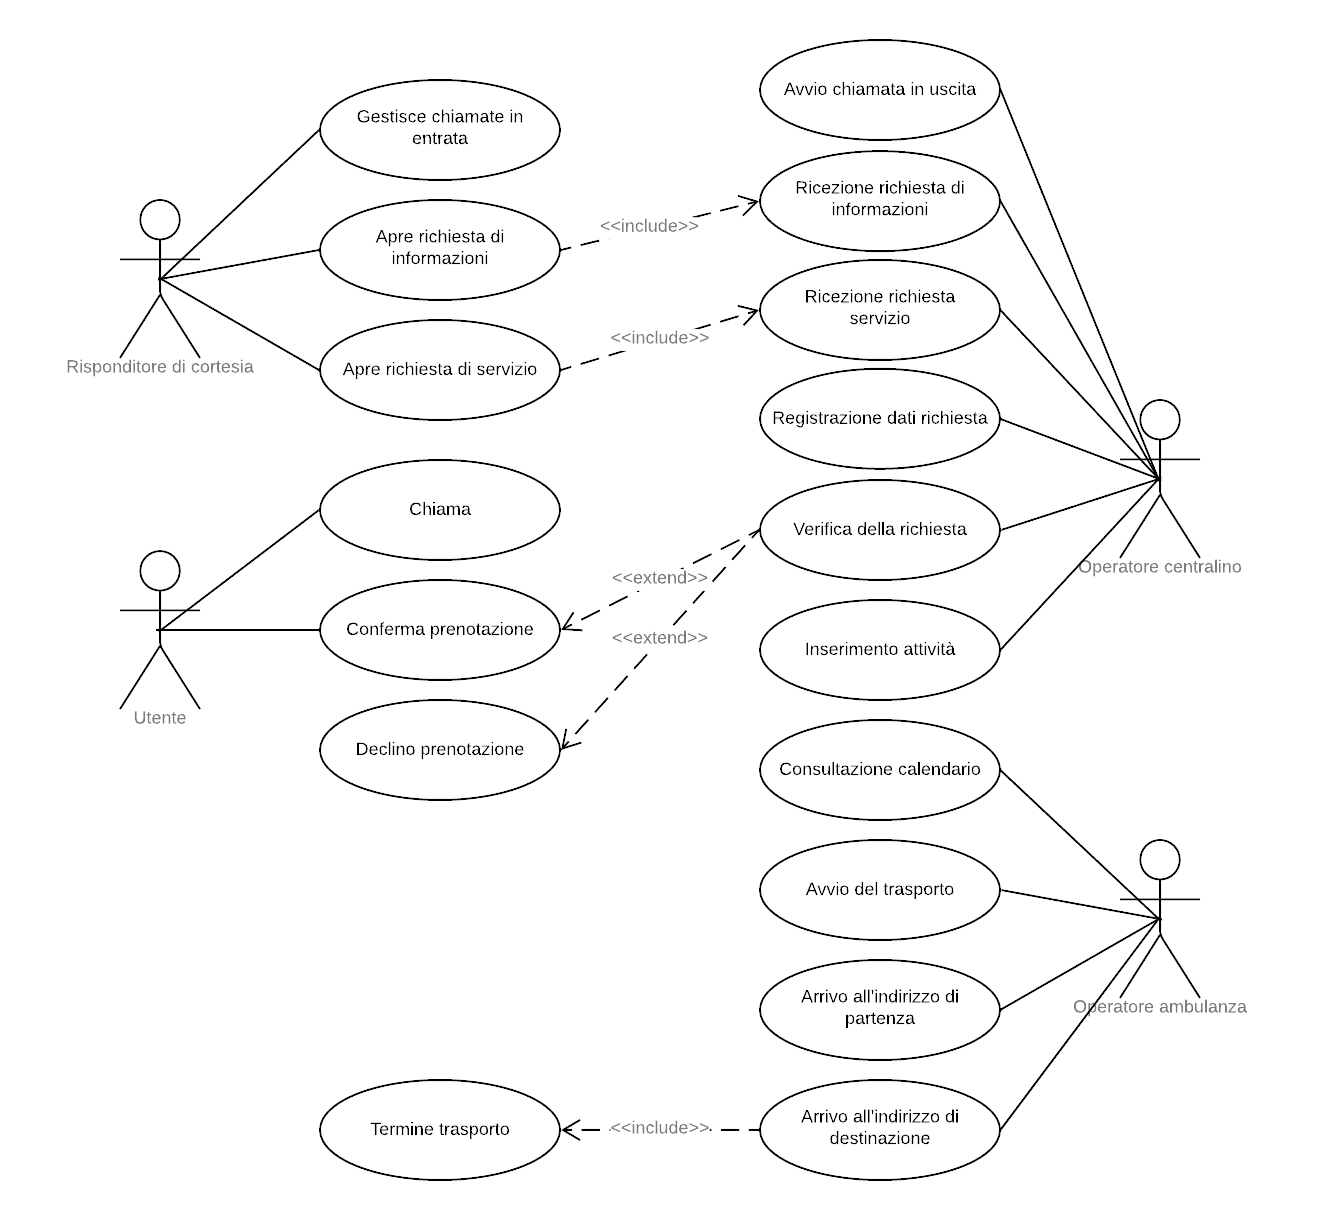
\includegraphics[width=13cm]{fig/Diagramma dei casi d'uso.png}
      \caption{Use case diagram}
      \label{use_case}
    \end{figure}
    
I requisiti del nuovo sistema evidenziati dall'esperto di dominio sono:
\begin{itemize}
    \item Il servizio 116117 è uno strumento di comunicazione che si rivolge a tutti i cittadini, italiani e stranieri, senza obbligo di registrazione preventiva.
    \item Il numero è unico in Italia ed in Europa.
    \item È un numero a chiamata rapida e non necessita di prefisso.
    \item Il numero è disponibile H24 per 7 giorni alla settimana.
    \item Fornisce assistenza e/o informazioni.
    \item Il servizio non è limitato nel tempo.
    \item Non è richiesto all'utente alcun pagamento per la chiamata.
    \item Le chiamate possono essere effettuate da qualunque apparecchio.
    \item \textbf{E’ auspicabile l’integrazione di soluzioni tecnologiche tra 118, 112 NUE e NE 116117} mantenendo comunque distinto l’accesso degli utenti alle due numerazioni, al fine di garantire affidabilità e sicurezza di funzionamento al sistema, presa in carico di chiamate provenienti da cittadini diversamente abili, fruibilità dei dati relativi ai pazienti da parte dei sanitari, utilizzo di sistemi di mediazione multilingue, registrazione informatizzata delle attività di localizzazione dei mezzi e di teletrasmissione.
   
    \item \textbf{Il corretto utilizzo dei sistemi di gestione automatica}. Nel centro di risposta NE 116117 non sono previsti sistemi di risposta automatica che chiudono la chiamata con un messaggio informativo né segreterie telefoniche, così come sistemi di istradamento delle chiamate entranti, possono essere previsti risponditori di cortesia o sistemi di messaggistica che informano il chiamante sui tempi previsti di attesa.
    \item \textbf{La gestione informatizzata dell'attività}. Registrazione vocale delle chiamate in entrata ed in uscita e loro archiviazione, con possibilità di riascolto delle registrazioni archiviate secondo le disposizioni in tema di sicurezza vigenti – anche al fine dell'elaborazione dei dati e dell'utilizzo di specifici indicatori che permettano di monitorare l’attività di servizio.
    \item \textbf{Governo delle centrali funzionalmente connesse nell'attività ordinaria ed emergenziale} ovvero: la centrale 118 per la risposta all'emergenza sanitaria e la centrale dei trasporti secondari.
    \item \textbf{Governo unico delle centrali 118 e 116117} che assicura un coordinamento omogeneo basato sull'esperienza maturata con la centrale unica Romagna 118 e che massimizza l’efficienza della risposta all'utente per situazioni di urgenza.
    \item Solida interfaccia tra la richiesta anche con \textbf{servizio di interpretariato} in caso di persone che non parlano italiano, e la struttura in grado di fornire la risposta, anche indiretta, alle esigenze dell'utente.
    \item \textbf{Infrastruttura tecnologica comune} che consente un'uniforme raccolta dati, base per l'analisi dei servizi erogati che permette di avere risposte pronte a specifici quesiti come di predisporre report periodici sull'attività svolta e la qualità degli interventi. 
    \item \textbf{Modellazione dell'ambulanza}. Si assume che tutte le ambulanze siano equipaggiate allo stesso modo, con un dispositivo per il tracciamento e un tablet per il controllo e la comunicazione con la centrale operativa. Così che, in caso di necessità, siano intercambiabili con quelle disponibili per il servizio 118.
    \item \textbf{Tracciamento dei percorsi al fine di analisi}. 
    \item \textbf{Storico degli eventi passati}. Si vuole tenere traccia dei trasporti passati, già conclusi al fine di future analisi ed eventuali necessità di controllo.
    \item \textbf{Registrazione di eventi di trasporto futuri}. Si vogliono memorizzare i trasporti prenotati per scopi organizzativi dell'occupazione dei mezzi e degli operatori.
    \item \textbf{Modellazione dell'operatore dell'ambulanza}.
    \item \textbf{Modellazione del paziente} al fine di mantenere traccia di tutti i servizi di cui ha usufruito in modo da poter effettuare opportune verifiche in caso di necessità.
    \item \textbf{Possibilità di fruizione dei dati da parte di sistemi esterni}.
\end{itemize}

 \begin{figure}[!ht]
    \centering
      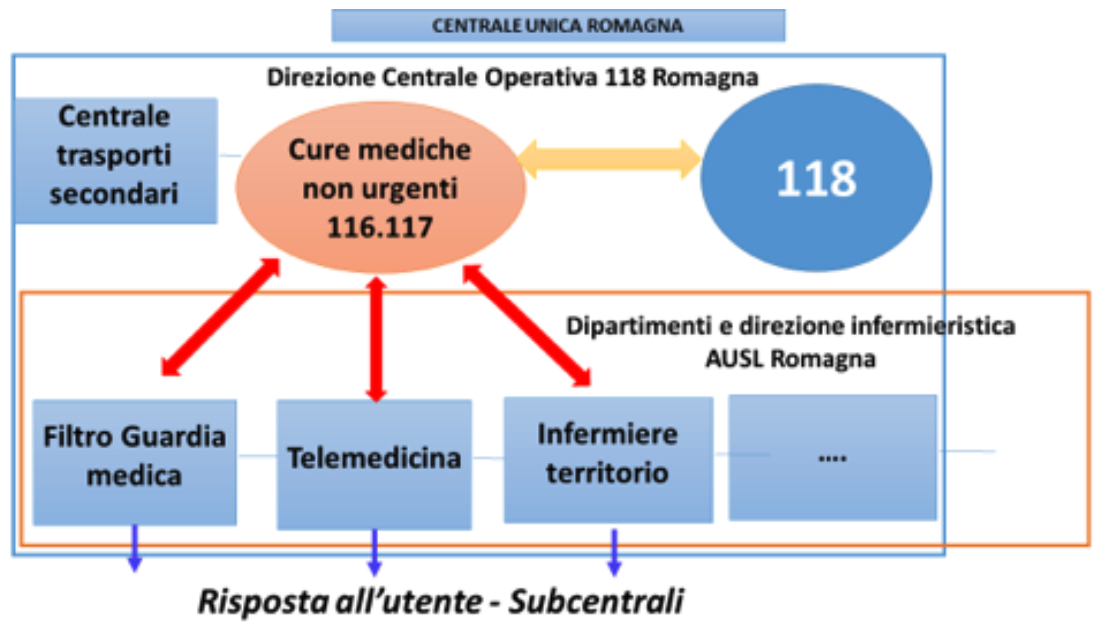
\includegraphics[width=13cm]{fig/org116117.png}
      \caption{Organizzazione interna 116117}
      \label{org}
    \end{figure}
    
     \begin{figure}[!ht]
    \centerline{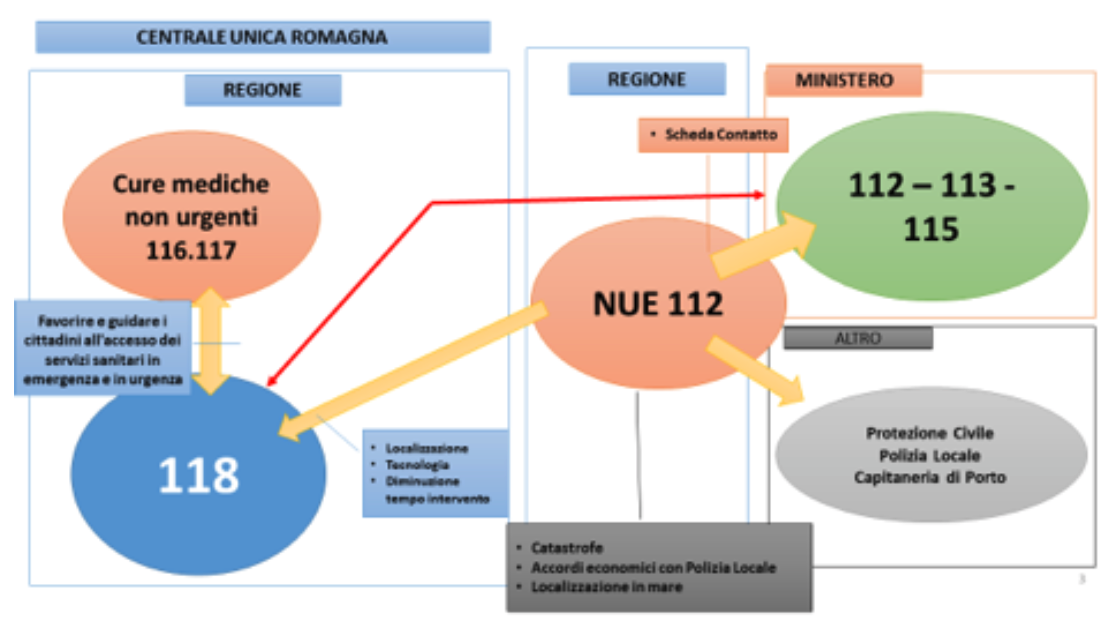
\includegraphics[width=13cm]{fig/comunicazione116117.png}}
      \caption{Comunicazione 116117, 118 e 112}
      \label{com}
    \end{figure}

\textbf{Considerazioni}
\begin{itemize}
    \item Si tiene traccia delle chiamate ricevute registrando i dati relativi alla chiamata e alla relativa richiesta anche nel caso in cui la prenotazione non andasse a buon fine, così da poter fare delle analisi sul servizio.
    \item La registrazione delle varie prenotazioni verrà segnata dall'operatore del centralino come nuova attività prevista nella giornata e sarà l’operatore dell'ambulanza a consultare attivamente ogni giorno le attività indicate.
    \item Il paziente, inteso come persona trasportata, non agisce attivamente all'interno del sistema ma, resta solamente un'entità passiva che subisce le azioni degli attori. Il paziente che agisce attivamente nel sistema (richiede il servizio) è incluso all'interno dell'attore “Utente”.
    \item Per ottimizzare l’utilizzo delle risorse disponibili, diversamente da quanto previsto nello scenario 3, si considerano gli eventi di andata e ritorno di un trasporto per trattamenti ricorrenti brevi, come due eventi distinti (come avviene nello scenario 4). In questo modo l’operatore non dovrà attendere la durata del trattamento e si potrà considerare libero per un'altra eventuale attività di trasporto. 
    \item \textbf{La tipologia delle informazioni e dei servizi}. Nell'elenco dei requisiti sottolineati dall'esperto del dominio emerge la necessità di avere distinzione delle figure all'interno del centralino per gestire i vari servizi offerti dal 116117. Nel nostro modello non sarà tenuto in considerazione questo aspetto poiché si fa riferimento solamente al servizio dei trasporti.
\end{itemize}

\subsection{Bounded Context e Context Map}

\centerline{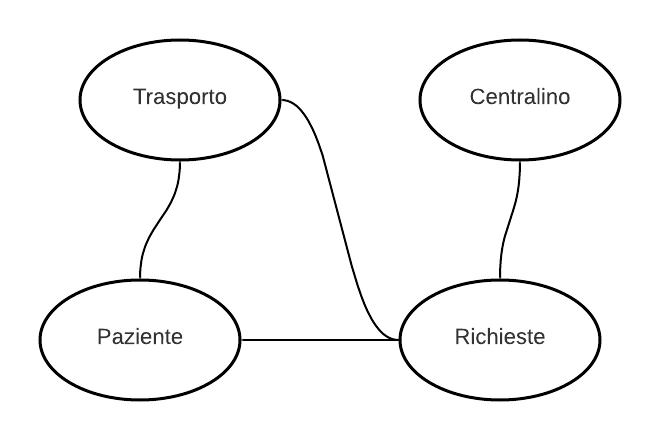
\includegraphics[width=13cm]{fig/ContextMap.png}}

L'immagine rappresenta i bounded context individuati durante l'analisi.
In particolare:
\begin{itemize}
    \item \textbf{Centralino}: bounded context che riguarda la ricezione della chiamata dell'utente da parte del centralino e la gestione della stessa, con l'eventuale trasferimento della chiamata ad un diverso operatore nel caso in cui si tratti di un utente che parla solamente una lingua specifica e l'eventuale attesa in coda nel caso in cui tutti gli operatori del centralino siano occupati.
    \item \textbf{Richieste}: parte del sistema relativa a tutte le richieste effettuate dagli utenti al centralino. In questo ambito sono incluse sia le richieste fatte ad unico scopo informativo, sia le richieste di poter usufruire del servizio. Da queste ultime, eventualmente, verrà poi effettuata la vera e propria prenotazione del trasporto.
    \item \textbf{Paziente}: bounded context in cui sono state racchiuse tutte le informazioni relative al paziente, compreso il suo stato di salute e il grado di autonomia, utile da conoscere per organizzare il trasporto.
    \item \textbf{Trasporto}: parte centrale del sistema che riguarda tutto il processo di trasporto. Include, infatti, l'itinerario da seguire, l'ambulanza utilizzata e l'operatore che si occupa dello specifico servizio.
\end{itemize}

\centerline{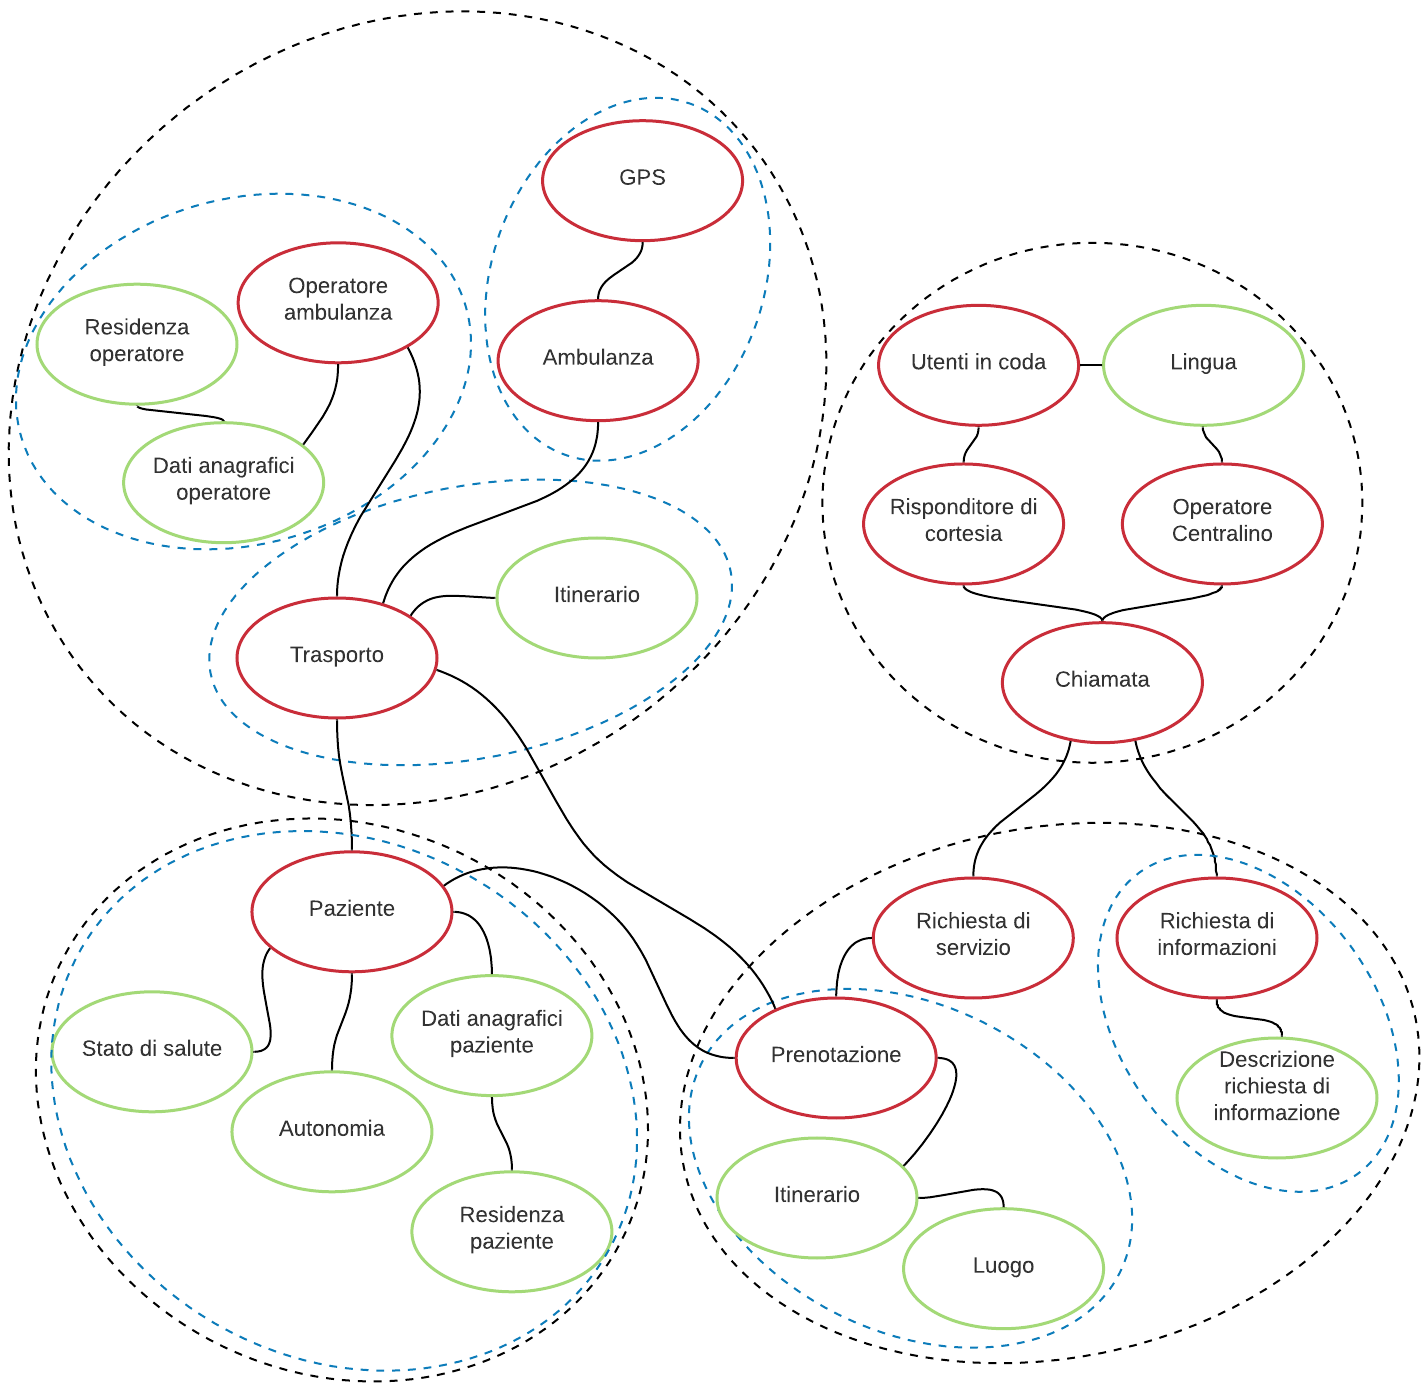
\includegraphics[width=15cm]{fig/BoundedContext.png}}

In figura si può vedere in dettaglio il contenuto, in termini di entità (evidenziate dal colore rosso) e relativi value object (evidenziate dal colore verde), dei bounded context individuati.
Inoltre, sono mostrati anche gli aggregati riconosciuti. In particolare, si vuole enfatizzare la presenza dell'aggregato contenente le due entità Ambulanza e GPS, in quanto sono due entità fortemente connesse poiché il GPS non potrebbe esistere senza la relativa ambulanza. Infatti l'entità ambulanza sarà l'unica entrata possibile nell'aggregato.

\section{Licenza Software}

Sono state utilizzate le API fornite da Microsoft Azure, vincolate da licenza MIT ma, poichè si tratta di una licenza estremamente permissiva e, soprattutto GPL compatibile, si è scelto di applicare al nostro software la GNU General Public License V. 3.

Abbiamo fatto questa scelta in quanto abbiamo ritenuto opportuno mantenere il software libero e open source ma, sottoposto ad un copyleft strong per cui il lavoro derivato da esso deve essere rilasciato sotto una licenza compatibile. Non può essere collegato ad un software a cui sono state applicate licenze che non siano compatibili con la GPLV3.

\section{Build automation}
L'applicazione delle tecniche di build automation hanno consentito di automatizzare la compilazione del codice e l'esecuzione dei test, nonché la gestione delle dipendenze ed il controllo di versione.

Abbiamo utilizzato diversi plugin a supporto del nostro progetto:
\begin{itemize}
    \item plugin relativi all'utilizzo del linguaggio Java;
    \item jUnit per il test del codice Java;
    \item jacoco per la coverage dei test. jacocoTestReport genera il report relativo alla coverage dei test eseguiti grazie al task di Test e fornisce il documento generato in formato html o xml;
    \item git-sensitive-semantic-versioning per la gestione delle versioni del software;
    \item javafx per la parte grafica dell'applicazione;
    \item java per la creazione automatica della javadoc.
\end{itemize}

Il progetto ha una struttura gerarchica che consta di tre sottoprogetti. Il primo relativo alle API messe a disposizione (\textit{digitalTwinAPI}) e i due restanti (\textit{ambulanceClient} e \textit{callCenterClient}) esempi di client che utilizzano le API create.
E\' stato definito un build.gradle comune a tutti i sottoprogetti, contenente tutto ciò che le tre parti hanno in comune: plug-in, dipendenze e funzionalità. Successivamente, il build.gradle di ogni sottoprogetto estende queste disponibilità con ciò che riguarda solamente la specifica parte.

\section{Versioning}
Per lo sviluppo delle API e i relativi client all'interno di questo progetto si è scelto di utilizzare il versioning semantico.

Il formato utilizzato è quindi \textbf{X.Y.Z} dove:
\begin{itemize}
    \item \textbf{X $\rightarrow$ Major}: incrementata con modifiche all'API pubblica che non sono compatibili con le versioni precedenti.
    \item \textbf{Y $\rightarrow$ Minor}: incrementata con l'introduzione di feature o miglioramento sostanziale del codice.
    \item \textbf{Z $\rightarrow$ Patch}: incrementata con la correzione di bug presente all'interno del codice.
\end{itemize}

\subsection{Git Flow}
Affiancato al processo di versioning si è deciso di utilizzare come flusso di sviluppo Git Flow, questo permette di mantenere un flusso di implementazione pulito.

I branch sono stati organizzati nel modo seguente:
\begin{itemize}
    \item \textbf{Master}: branch contenente la storia delle release ufficiali.
    \item \textbf{Develop}: branch contenente la linea di sviluppo, contiene tutte le feature completate. Da questo branch partiranno i branch \textit{feature} e \textit{bug-fix}.
    \item \textbf{Feature}: branch contenente una nuova feature in via di sviluppo. 
    \item \textbf{Bug-fix}: branch utilizzato per la risoluzione di un bug. Può partire sia dal branch \textit{develop} che da un branch \textit{feature}.
\end{itemize}

\section{Validazione e Test}

\subsection{Testing automatizzato}
Lo sviluppo dei servizi forniti ai client è stato testato mediante la libreria JUnit. 
Il progetto è stato testato in modo automatico mediante l'utilizzo di Travis CI. 
Avendo, però, tramite travis-ci.com una serie limitata di build e dato che dal 15 giugno 2021, la build su travis-ci.org è cessata, si è pensato di utilizzare GitHub Actions per la continuos integration.
Tramite GitHub Actions si eseguono in maniera automatica i test su Windows. Non è stato ritenuto necessario testare il sistema anche su altri OS in quanto un vincolo presente all'interno del sistema sanitario italiano è quello di utilizzare sistemi operativi Windows.

All'interno del progetto sono presenti le seguenti classi di test:
\begin{itemize}
    \item AmbulanceIdGeneration: testa la generazione degli id di ambulanza e GPS.
    \item DtAmbulance: testa i servizi relativi al digital twin dell'ambulanza.
    \item DtBookingTransport: testa i servizi relativi al digital twin della prenotazione.
    \item DtConnection: testa la connessione al client.
    \item DtInfoRequest: testa i servizi relativi al digital twin della richiesta di informazioni.
    \item DtOperator: testa i servizi relativi al digital twin dell'operatore.
    \item DtPatient: testa i servizi relativi al digital twin del paziente.
    \item DtServiceRequest: testa i servizi relativi al digital twin della richiesta di servizio.
    \item DtTransport: testa i servizi relativi al digital twin del trasporto.
\end{itemize}

\subsection{Implementazione Scenari}\label{sez62}
\subsubsection{Scenario 1}
L'operatore che riceve la chiamata inserisce nel sistema il nuovo paziente e la prenotazione, tramite il Call Center Client. Nell'immagine seguente si può vedere l'inserimento della prenotazione e del paziente, poiché non era ancora all'interno del sistema. 

\hfill \break

\centerline{
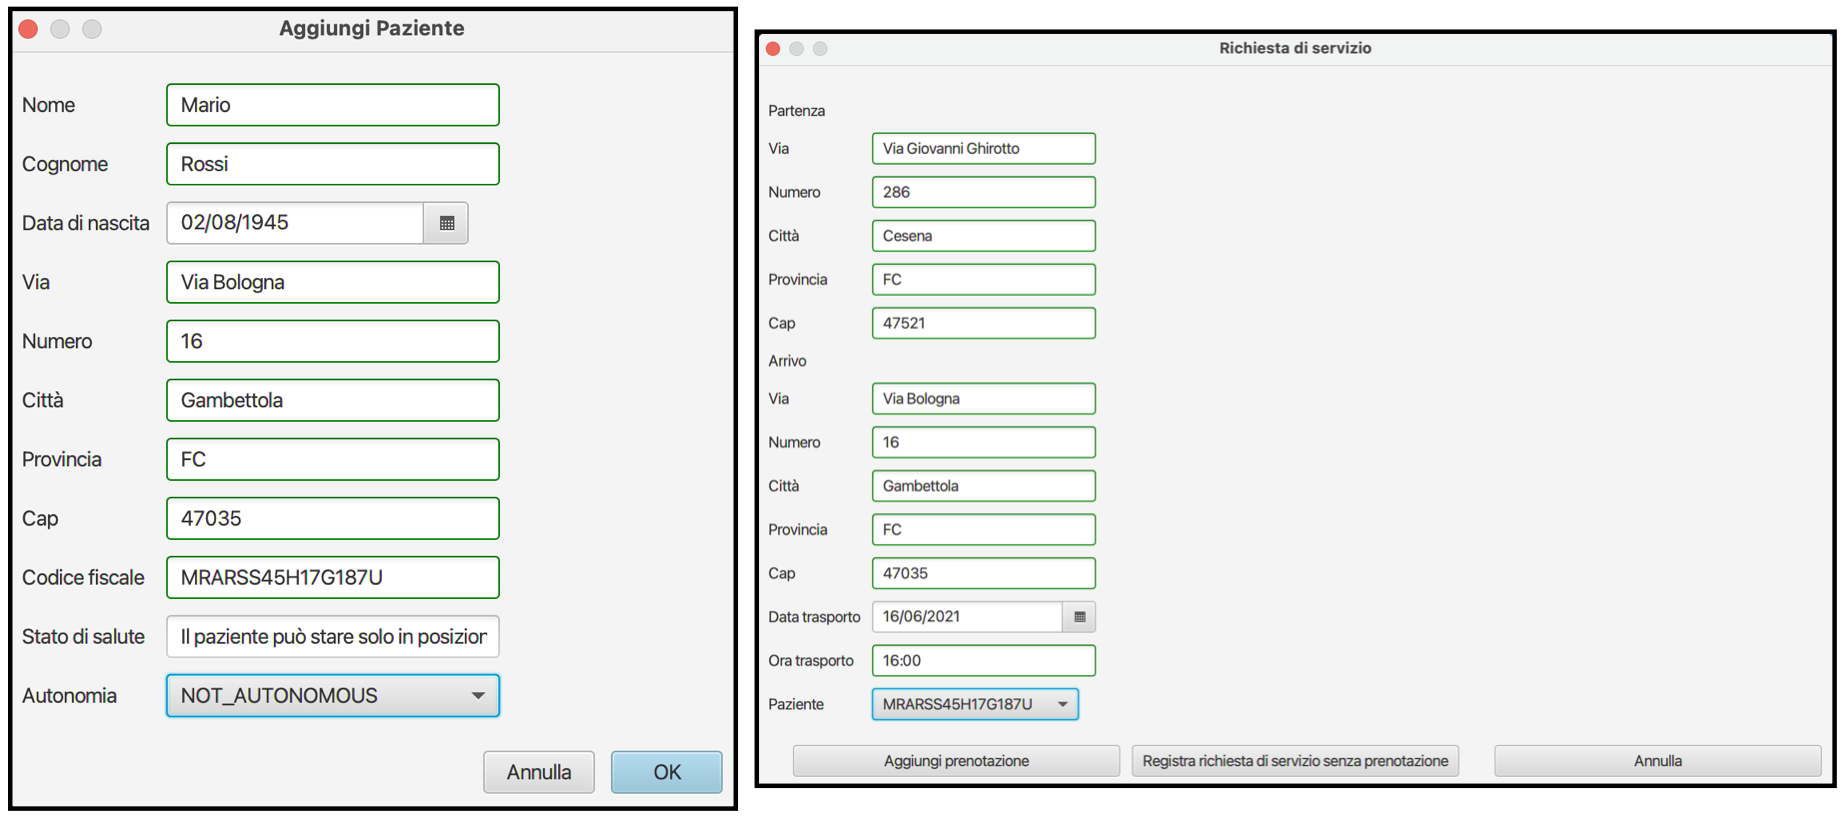
\includegraphics[width=15cm]{fig/Prenotazione.png}}
\hfill \break


Nella figura seguente è riportato il digital twin graph dopo l'inserimento di questi dati:
\hfill \break

\centerline{
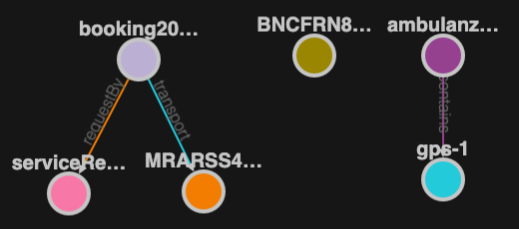
\includegraphics[width=13cm]{fig/scenario1-prenotazione.png}}
\hfill \break

 L'operatore controlla le prenotazioni per la giornata dall'Ambulance client.
 Successivamente, seleziona la prenotazione e conferma la presa in carico del trasporto come nella figura seguente:
 \hfill \break

\centerline{
 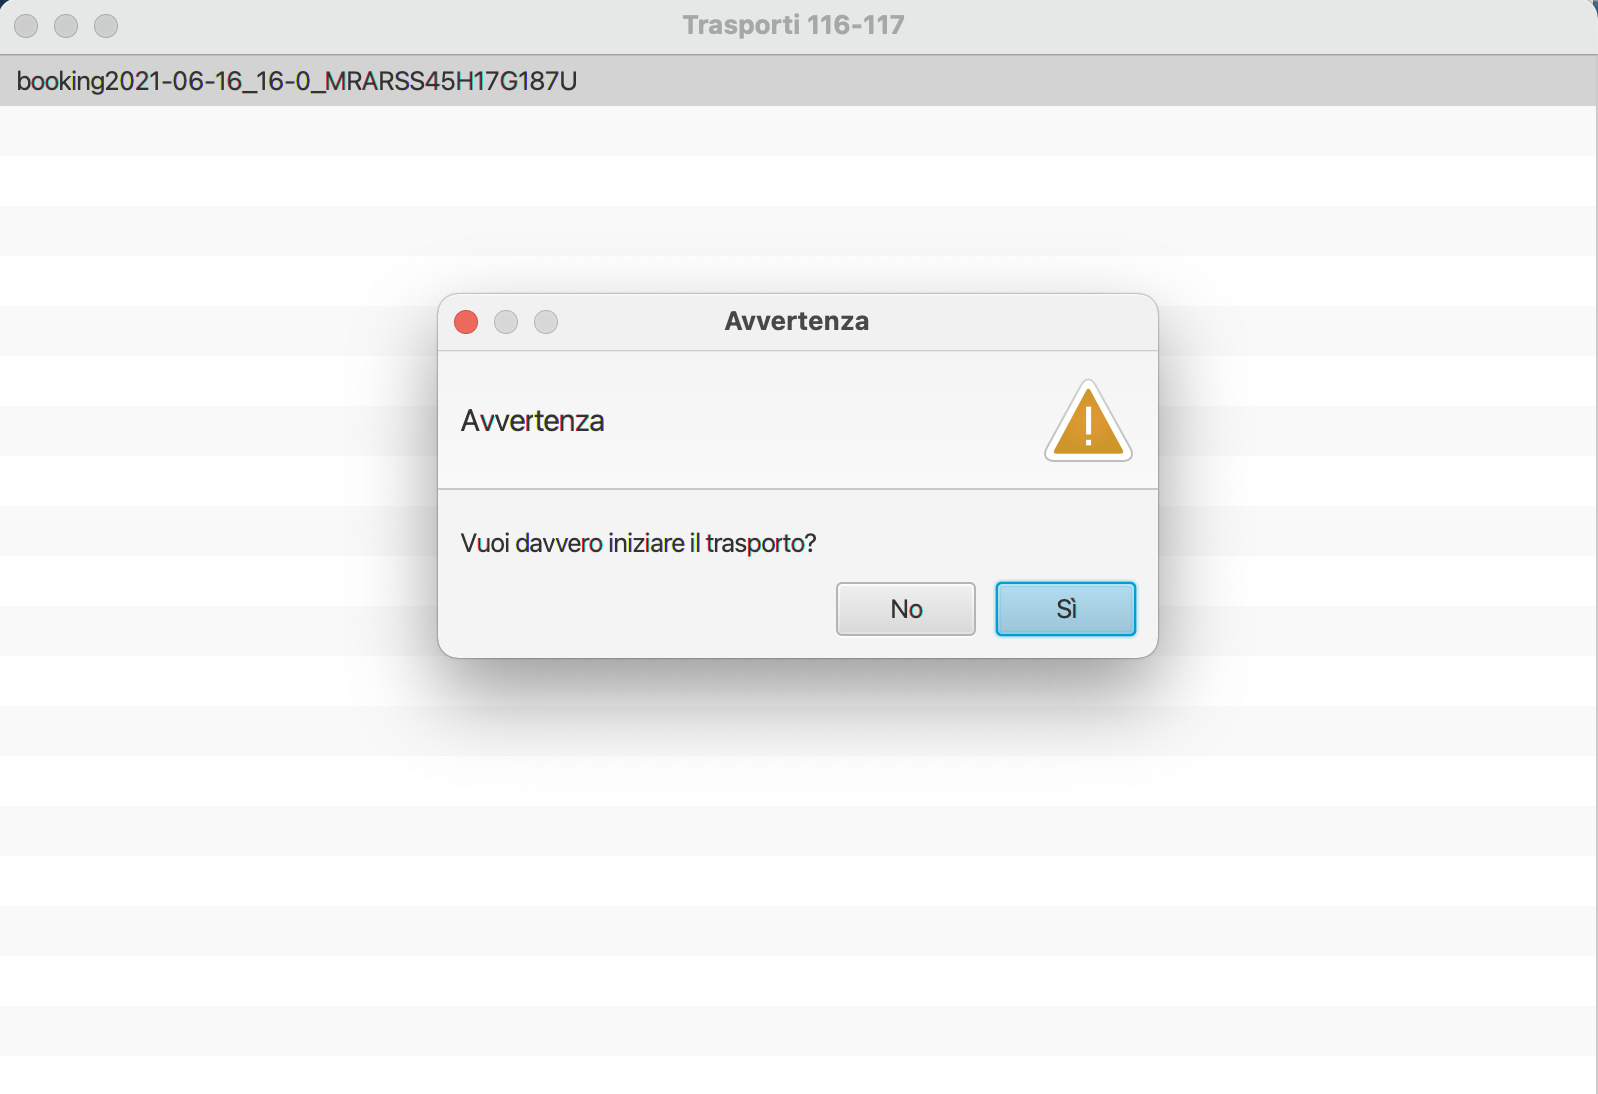
\includegraphics[width=13cm]{fig/prenotazioni.png}}
\hfill \break

 A questo punto esegue il trasporto. 
 Giunto a destinazione, dopo avere lasciato il paziente a destinazione, termina il trasporto.
 In figura si può vedere il digital twin graph al termine dello scenario 1.
 \hfill \break
 
 \centerline{
 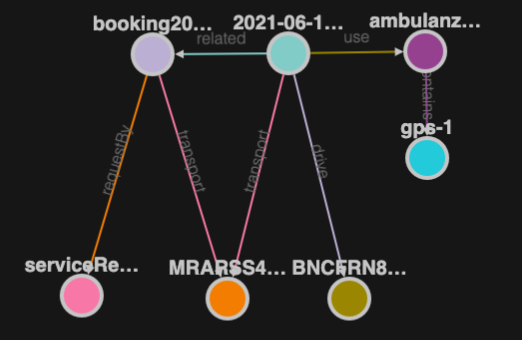
\includegraphics[width=12cm]{fig/scenario1-fine.png}}
\hfill \break

\subsubsection{Altri scenari}
La simulazione degli altri 3 scenari è risultata pressoché uguale allo scenario 1. Durante le simulazioni non sono emersi problemi rilevanti.

Durante lo svolgimento delle simulazioni è sorta, però, una possibile ottimizzazione da svolgere negli sviluppi futuri: le prenotazioni potrebbero essere proposte all'operatore dell'ambulanza in ordine di vicinanza al mezzo che sta utilizzando, in modo da ottimizzare lo sfruttamento dei mezzi e degli operatori. 

\subsection{Test Coverage}
 \centerline{
 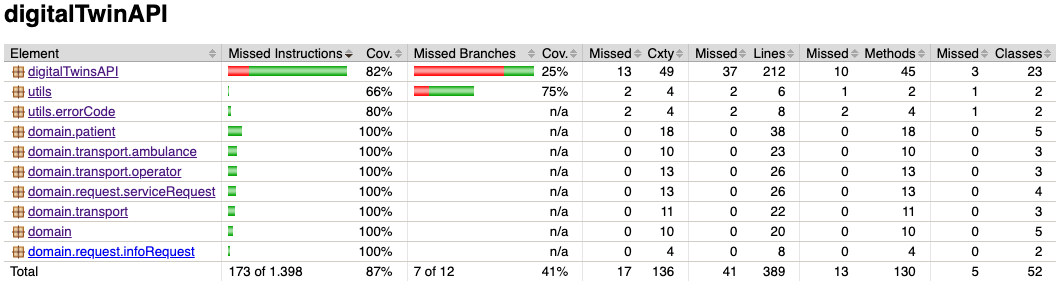
\includegraphics[width=18cm]{fig/testCoverage.png}}
\hfill \break

Come si evince in figura, è riportata solamente la coverage relativa al sub-project \textit{digitalTwinAPI}. Infatti si è deciso di validare le parti relative agli altri due sub-project \textit{ambulanceClient} e \textit{callCenterClient} non tramite JUnit Test, ma manualmente tramite l'implementazione degli scenari individuati nella fase di knowledge crunching, come riportato nella sezione \ref{sez62}.  

Si è ritenuto che la parte fondamentale da testare fosse la parte relativa alle API fornite, ovvero il sub-project \textit{digitalTwinAPI}. 

Come si può vedere sopra, nei test relativi a questo sub-project si è raggiunta una coverage del 87\%. Il risultato è stato considerato soddisfacente.

\section{Miglioramenti futuri}

\centerline{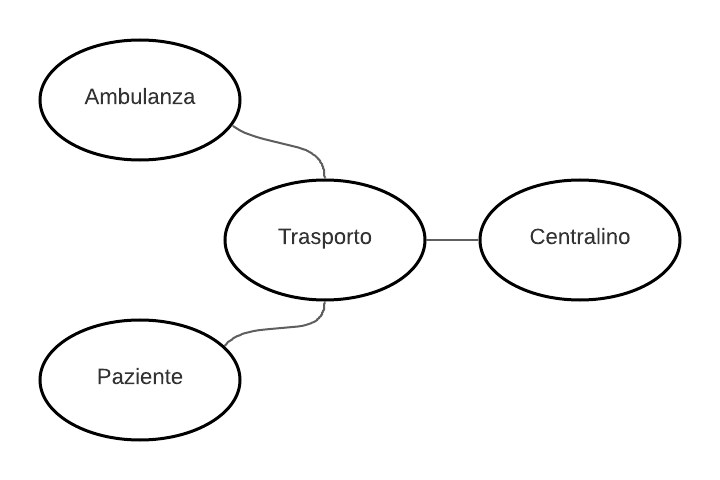
\includegraphics[width=13cm]{fig/ContextMap2.png}}
Come mostrato in figura, data la forte indipendenza dell'aggregato relativo all'ambulanza e quello relativo all'operatore della stessa, attualmente parte del bounded context del trasporto, si potrebbero esportare da quest'ultimo, per introdurre un nuovo bounded context apposito.
Inoltre, il bounded context relativo alle richieste è stato collassato all'interno del bounded context del trasporto in quanto si considerano le richieste e le prenotazioni, come fasi in cui si può trovare il processo del trasporto.

\centerline{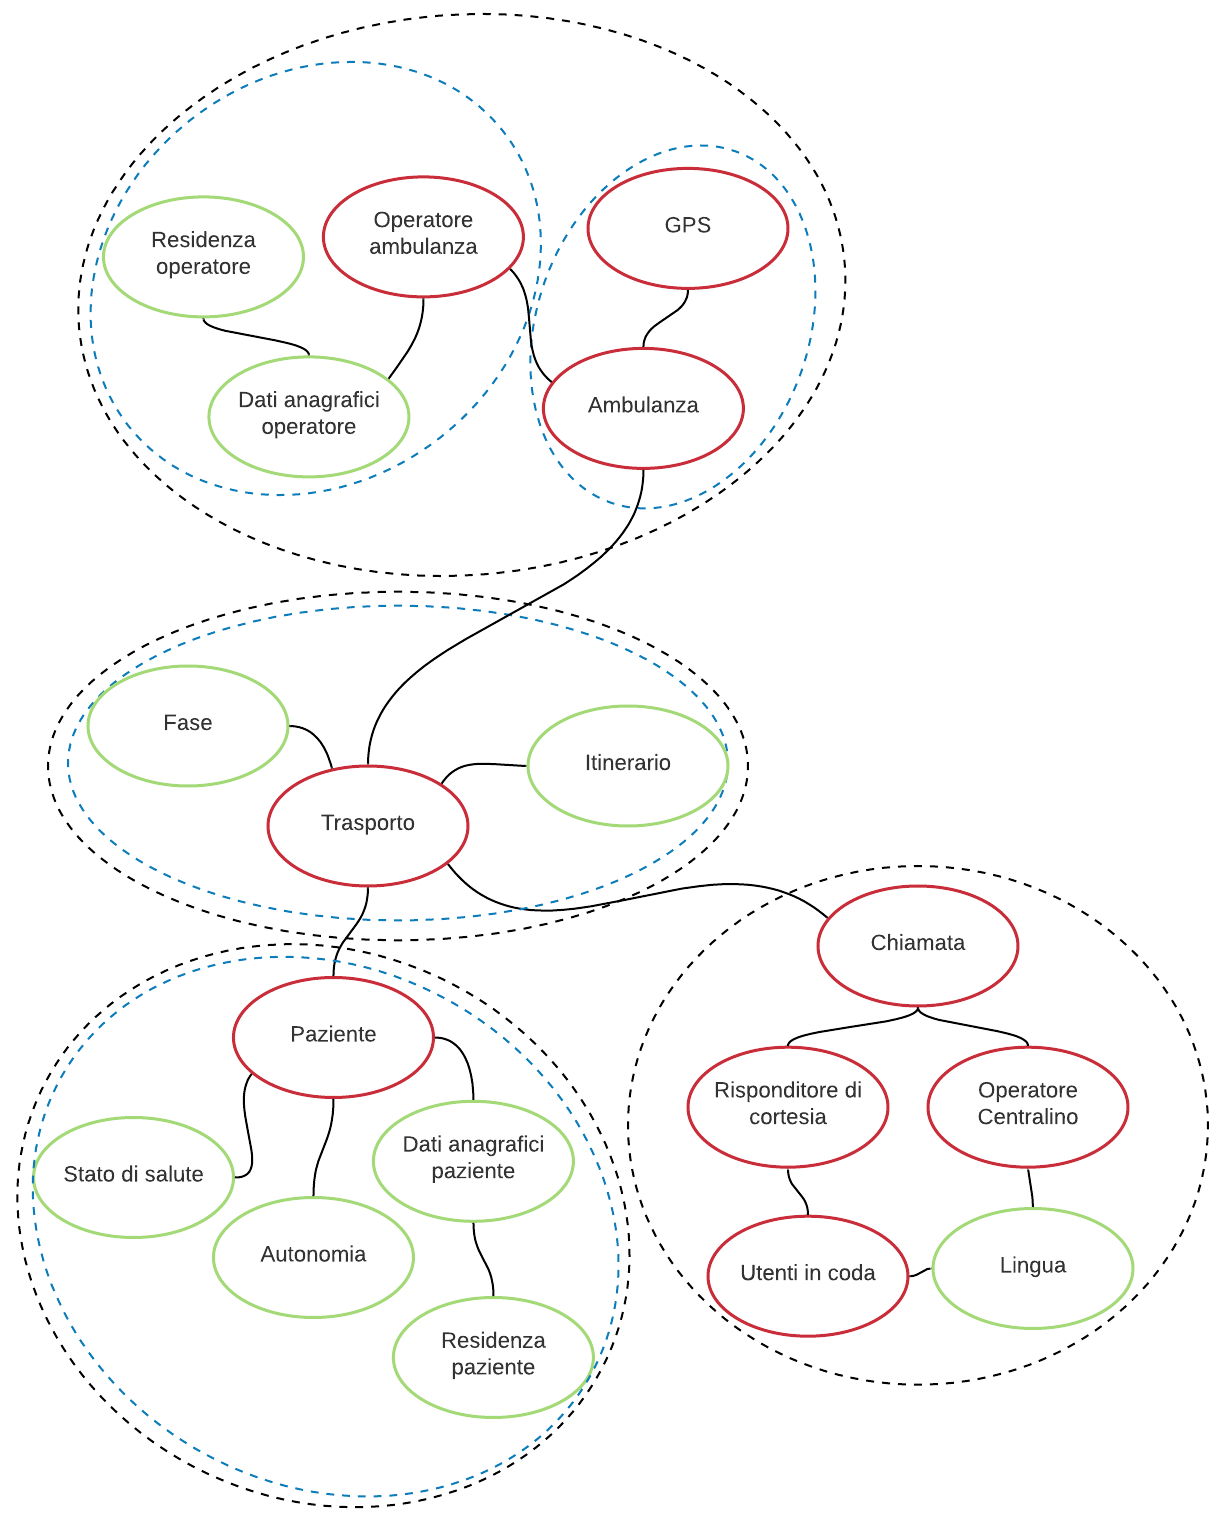
\includegraphics[width=15cm]{fig/BoundedContext2.png}}

In figura è mostrata la nuova organizzazione relativa alle entità ed ai value object all'interno dei diversi bounded context, rispetto all'individuazione di un nuovo bounded context ed alla modifica di quelli presenti in precedenza. 


\section{Integrazione Elaborato}
\subsection{Build Automation}
\subsubsection{Processo di QA}
Per il processo di QA sono stati utilizzati i seguenti strumenti:
\begin{itemize}
    \item\textbf{Checkstyle}: è stata utilizzata la configurazione che segue le Sun Code Conventions. Da questa configurazione sono stati tolti alcuni moduli che abbiamo ritenuto non in linea con il nostro progetto, pur rispettando le best practices di Java. Una di queste è quella relativa ai magic number, poichè nei form all'interno della GUI è utilizzato un GridPane e Checkstyle chiedeva di sostituire gli svariati indici per il posizionamento degli elementi con costanti. Abbiamo riscontrato una migliore leggibilità del codice senza l'utilizzo di costanti.
    
    \item \textbf{PMD}: sono stati utilizzati due rule sets standard, ovvero: errorProne e bestPractices. Gli ulteriori rule sets standard non sono stati inclusi poiché alcuni erano in sovrapposizione con l'analisi svolta da checkstyle mentre altri non erano utili al fine del progetto.
    Inoltre, è stata impostato il parametro rulesMinimumPriority a 4 anziché a 5 (equivalente ad un consiglio di modifica altamente opzionale).
\end{itemize}

\subsubsection{Shadow JAR}
Per la creazioni dei due jar relativi a ambulanceClient e callCenterClient è stato utilizzato Shadow Jar.
Questo plug-in permette, appunto, la creazione di fat jar, ovvero jar eseguibili che contengono, oltre le classi compilate, anche tutte le dipendenze del progetto. 

\subsection{Continuos Integration}
Il workflow viene eseguito solo quando vengono effettuati push sul branch master e develop, quando viene aggiunto un tag e, in ogni caso, alla mezzanotte del primo giorno di ogni mese. 

\subsubsection{Controllo sottoscrizione Azure}
Il job \textbf{AzureJob} si occupa di controllare lo stato della sottoscrizione di Azure.
Tramite la CLI di Azure effettua la connessione al portale: per effettuare il login utilizza il client secret dell'applicazione registrata su Azure Active Directory, lo stesso metodo utilizzato dall'applicazione Java.

La risposta ricevuta dalla richiesta di connessione contiene diverse informazioni relative alla sottoscrizione. Tra queste si può estrapolare lo stato (abilitato o disabilitato) della sottoscrizione per poi inserirlo in una variabile che permetterà al job di test, \textbf{GradleJob}, di distinguere tra due diversi comandi da eseguire: il test completo dell'applicazione o i task relativi alla quality assurance del codice.

\subsubsection{Integrazione build}
All'interno di \textbf{GradleJob} vengono eseguiti i test e i controlli di QA. Questo job si serve dell'output generato dall'esecuzione del job precedente per eseguire due processi diversi nel caso in cui la sottoscrizione sia attiva o meno: in caso affermativo effettua sia i test che il processo di QA, in caso negativo effettua solo il processo di QA.
In quest'ultimo caso, si è scelto di non svolgere i test poiché essi sono tutti dipendenti da Azure. 

Le operazioni effettuate da questo job vengono eseguite su sistemi operativi MacOs, Linux e Ubuntu per le versioni 11, 14, 16 di Java. Le varie run vengono eseguite sequenzialmente, questo serve poiché durante i test si vanno a creare e ad eliminare, all'interno dell'ambiente Azure, dei Digital Twin di prova che causerebbero una sovrapposizione all'interno dell'ambiente che potrebbe portare ad un comportamento imprevedibile dei test.

\subsubsection{Sincronizzazione con Overleaf e compilazione}
Per avere sempre un report aggiornato è stato sincronizzato il progetto Overleaf al repository. Questo permette di fare il push delle modifiche al report, ogni volta che si ritenga necessario, direttamente da Overleaf.

Tramite le Github Actions è stato creato un job che si occupa, successivamente, della compilazione del codice Latex e la produzione del pdf relativo. Questo artefatto verrà poi inserito all'interno della release.

\subsubsection{Creazione automatica dalla release}
Il job \textbf{Release} è dipendente da \textbf{GradleJob}, questo assicura il corretto funzionamento della release. Il job viene eseguito ogni qual volta viene effettuato un tag. Per ogni tag, quindi, creerà una release contenente il source code, la licenza, il report e i due jar eseguibili relativi ai client. Prima di creare la release, infatti, vengono creati i jar tramite il task di gradle \textit{shadowJar}.

\end{document}